%\documentclass[11pt]{article}
%\usepackage{graphicx}
%\usepackage{amsmath,amssymb, amsthm}
%\usepackage{color}
%%\usepackage[hidelinks]{hyperref}
%\usepackage{hyperref}
% \usepackage{amsfonts}
% \usepackage{makeidx}
% \usepackage{xfrac}
% % \usepackage{ulem}
% \usepackage{tikz}
% \usetikzlibrary{arrows}
% \usepackage{natbib}
% %\bibliographystyle{chicagoa}
% \makeindex
%      
%\textwidth = 6.5 in \textheight = 8.5 in \oddsidemargin = 0.0 in
%\evensidemargin = 0.0 in \topmargin = 0.0 in \headheight = 0.2 in
%\headsep = 0.5 in
%\parskip = 0.2in
%\parindent = 0.2in
%
%\newcommand{\cyp}{\citeyearpar}
%\newcommand{\ha}{\frac{1}{2}}
%\newcommand{\R}{\mathbb{R}}
%\newcommand{\C}{\mathbb{C}}
%\newcommand{\CP}{\mathbb{CP}}
%\newcommand{\RP}{\mathbb{RP}}
%\newcommand{\PP}{\mathbb{P}}
%\newcommand{\N}{\mathbb{N}}
%\newcommand{\Q}{\mathbb{Q}}
%\newcommand{\Z}{\mathbb{Z}}
%\newcommand{\B}{\mathbb{B}}
%\newcommand{\A}{\mathbb{A}}
%\newcommand{\Hom}{\rm{Hom}}
%\newcommand{\F}{\mathbb{F}}
%\newcommand{\ii}{\sqrt{-1}}
%\newcommand{\ph}{\varphi}
%\newcommand{\rd}{\partial}
%\newcommand{\dux}{\frac{\partial u}{\partial x}}
%\newcommand{\duy}{\frac{\partial u}{\partial y}}
%\newcommand{\dvx}{\frac{\partial v}{\partial x}}
%\newcommand{\dvy}{\frac{\partial v}{\partial y}}
%\newcommand{\ulr}{\underline{r}}
%\newcommand{\ulu}{\underline{u}}
%\newcommand{\ulv}{\underline{v}}
%\newcommand{\ulg}{\underline{g}}
%\newcommand{\ulga}{\underline{\gamma}}
%\newcommand{\olb}{\overline{\B}}
%\newcommand{\dsp}{\displaystyle}
%\newcommand{\gdg}{\emph{Grundlagen der Geometrie}}
%\newcommand{\n }{^{-1}}
%\newcommand{\rr}{\mathbf{r}}
%\newcommand{\col}{\textcolor}
%\newcommand{\ci}{\mathcal{I}}
%\newcommand{\cz}{\mathcal{Z}}
%\newlength{\wdth}
%\newcommand{\strike}[1]{\settowidth{\wdth}{#1}\rlap{\rule[.5ex]{\wdth}{.4pt}}#1}
%
%
%\newcommand{\mm}{$\mathbf{m}$}
%\newcommand{\rrt}{Riemann--Roch Theorem}
%\newcommand{\dieq}{dialytic equation}
%\newcommand{\chnr}{characteristic number}
%\newcommand{\moeq}{modular equation}
%\newcommand{\nft}{Noether's Fundamental Theorem}
%\newcommand{\cbt}{Cayley--Bacharach theorem}
%
%\def\PP{{\mathbb P}}
%
%\newtheorem{theorem}{Theorem}
%\newtheorem{lemma}{Lemma}
%\newtheorem{corollary}[theorem]{Corollary}
%\newtheorem{definition}{Definition}
%\newtheorem{example}{Example}
%\raggedbottom
%
%\def\de#1{{{\bf \col{red}{David says [* }\col{red}{#1{\bf\ *]} }}}}
%\def\fix#1{{{\bf \col{red}{Jeremy says [* }\col{red}{#1{\bf\ *]} }}}}
%


%\begin{document}
%header and footer for separate chapter files

\ifx\whole\undefined
\documentclass[12pt, leqno]{book}
\usepackage{graphicx}
\input style-for-curves.sty
\usepackage{hyperref}
\usepackage{showkeys} %This shows the labels.
%\usepackage{SLAG,msribib,local}
%\usepackage{amsmath,amscd,amsthm,amssymb,amsxtra,latexsym,epsfig,epic,graphics}
%\usepackage[matrix,arrow,curve]{xy}
%\usepackage{graphicx}
%\usepackage{diagrams}
%
%%\usepackage{amsrefs}
%%%%%%%%%%%%%%%%%%%%%%%%%%%%%%%%%%%%%%%%%%
%%\textwidth16cm
%%\textheight20cm
%%\topmargin-2cm
%\oddsidemargin.8cm
%\evensidemargin1cm
%
%%%%%%Definitions
%\input preamble.tex
%\input style-for-curves.sty
%\def\TU{{\bf U}}
%\def\AA{{\mathbb A}}
%\def\BB{{\mathbb B}}
%\def\CC{{\mathbb C}}
%\def\QQ{{\mathbb Q}}
%\def\RR{{\mathbb R}}
%\def\facet{{\bf facet}}
%\def\image{{\rm image}}
%\def\cE{{\cal E}}
%\def\cF{{\cal F}}
%\def\cG{{\cal G}}
%\def\cH{{\cal H}}
%\def\cHom{{{\cal H}om}}
%\def\h{{\rm h}}
% \def\bs{{Boij-S\"oderberg{} }}
%
%\makeatletter
%\def\Ddots{\mathinner{\mkern1mu\raise\p@
%\vbox{\kern7\p@\hbox{.}}\mkern2mu
%\raise4\p@\hbox{.}\mkern2mu\raise7\p@\hbox{.}\mkern1mu}}
%\makeatother

%%
%\pagestyle{myheadings}

%\input style-for-curves.tex
%\documentclass{cambridge7A}
%\usepackage{hatcher_revised} 
%\usepackage{3264}
   
\errorcontextlines=1000
%\usepackage{makeidx}
\let\see\relax
\usepackage{makeidx}
\makeindex
% \index{word} in the doc; \index{variety!algebraic} gives variety, algebraic
% PUT a % after each \index{***}

\overfullrule=5pt
\catcode`\@\active
\def@{\mskip1.5mu} %produce a small space in math with an @

\title{Personalities of Curves}
\author{\copyright David Eisenbud and Joe Harris}
%%\includeonly{%
%0-intro,01-ChowRingDogma,02-FirstExamples,03-Grassmannians,04-GeneralGrassmannians
%,05-VectorBundlesAndChernClasses,06-LinesOnHypersurfaces,07-SingularElementsOfLinearSeries,
%08-ParameterSpaces,
%bib
%}

\date{\today}
%%\date{}
%\title{Curves}
%%{\normalsize ***Preliminary Version***}} 
%\author{David Eisenbud and Joe Harris }
%
%\begin{document}

\begin{document}
\maketitle

\pagenumbering{roman}
\setcounter{page}{5}
%\begin{5}
%\end{5}
\pagenumbering{arabic}
\tableofcontents
\fi


\chapter{A historical essay on some topics in algebraic geometry}
This essay offers a brief overview of aspects of the long history of plane curves and algebraic geometry.\footnote{I am grateful to Andrea del Centina for letting me read the manuscript of his forthcoming book \emph{The History of Projective Geometry}, which has been very helpful and will surely become the definitive work on the subject.}   It starts with some historical remarks about conic sections, moves on to look some aspects of the early study of cubic and quartic curves and the emergence of real and complex projective space, then nods briefly at Riemann's ideas about algebraic curves and Cremona's ideas about plane transformations before concluding with an introduction to the work of Brill and Noether in the late 19th century. 

\section{Greek mathematicians and conic sections}
Quadratic problems were part of high-level teaching in ancient Mesopotamia around 1800 BCE. One such tablet (BM 13901) begins 
\begin{quote}
I have added up the area and the side of my square: 0;45.
\end{quote}
The unstated task is to find the side of the square.
The number 0;45 is $\frac{3}{4}$ in sexagesimal notation, so if we rewrite this as an equation for $s$, the unknown side, we have
\[s^2 + s = \frac{3}{4}.\]
The tablet then goes through the steps of an algorithm much as we would for finding the positive root: $s = \frac{1}{2}.$ 

Other problems involve knowledge of the Pythagorean theorem, known also to Chinese and Indian mathematicians. But the first mathematicians to have studied curves more complicated than the straight line and the circle seem to have been those of ancient Greece.  Surviving sources suggest that the study of conic sections, literally sections of a cone, may well have arisen with Menaechmus's work on doubling the cube around 350 BCE. This was a long-standing problem that was given a theological spin in the form of the Delian problem, which, according to one story, asked for an altar double the size of a given one, apparently to get rid of a plague. Finding this difficult, workers consulted Plato, who said that the real reason for the task was to reproach the Greeks for their neglect of geometry.\footnote{Theon of Smyrna, 2nd century CE, in (Thomas 1939, Vol. 1, 257).}
It may well also have stood out because Plato in the \emph{Meno} dialogue made such a fuss of doubling the square. Hippocrates of Chios, who flourished around 470 BCE,  had already reduced the problem to that of finding two mean proportionals between 1 and 2; i.e. quantities $x$ and $y$ such that 
\begin{equation}~\label{Menmus}
1:x= x:y = y: 2.
\end{equation}
For Greek mathematicians, these would have been line segments of those lengths. 

Many solutions to the problem of finding two mean proportionals were propose, a younger associate of Plato and a pupil of Eudoxus, may have been the first to connect the problem of doubling the cube to the idea of conic sections, or perhaps we should say quadratic curves, because it has been argued that he considered equation \eqref{Menmus} as defining or generating curves that would have been drawn and understood pointwise. At all events, he expressed the solution to the Delian problem in terms of the intersection of a hyperbola and a parabola.\footnote{See Eutocius \emph{Commentary on Archimedes' Sphere and Cylinder}, in (Cohen and Drabkin 1948, 62--66). Among Eudoxus's many achievements is to have provided the first theory of magnitudes that went beyond the rational numbers; it is now found in Book V of Euclid's \emph{Elements}.}

About a century after Menaechmus, Diocles, and soon after him Apollonius, made significant progress with the conic sections.\footnote{In many ways, the first place to go for an account of Greek mathematics remains Sir T.L. Heath's century-old account (Heath 1921), but it should be supplemented by more modern readings, such as (Knorr  1993).}
Diocles identified the curve that would focus the sun's rays to a point as the parabola, and knew precisely how to cut a cone so as to obtain it.\footnote{Apollonius's four books of his conics survive in Greek and three more in Arabic; the eighth and final volume is lost.} 


Apollonius produced the first \emph{theory} of conic sections as sections of a cone. 
The books are very dry. Van der Waerden called him a virtuoso ``in dealing with geometric algebra, and also a virtuoso in hiding his original line of thought'', while going on to say that ``his reasoning was crystal clear and elegant.''\footnote{See (Van der Waerden 1961, 248).}
He began with the basic definitions of a cone (on a circle) and its three types of section: the hyperbola, parabola, and ellipse; the names are due to him. He showed that all the known sections that had been studied as sections of a cone with vertical angle a right angle could be obtained as sections of a suitable but otherwise arbitrary cone.

It's  arguable that a system of coordinates was present in his work, inasmuch as he generally referred everything to a pair of distinguished lines in the plane of section of the cone, but it is buried in the heavy use of proportion theory between different line segments. 
Apollonius produced a theory of the principal diameters of conics, studied such problems as finding the tangents to a conic from an exterior point, and came close to observing the properties of cross-ratio that modern writers were to detect. He also had a theory about normals to conics from which  it's a short step to obtaining their evolutes. 
The biggest weakness in his theory was that very often he had to treat the three kinds of conic section separately, although you can see him trying for greater generality. 




Mathematicians of the Islamic era  also studied conic sections and the various problems they inherited from the Greeks. One of the most outstanding is `Umar ibn Ibr\={a}h\={i}m al-Kh\={a}yyam\={i} (usually known in the West as Omar Khayy\={a}m), who was born in Nishapur in northern Iran  in the 11th century CE and spent much of his life in Isfahan where he led a group of Islamic astronomers at the observatory there. In his book the \emph{Ris\={a}la} he 
 gave a complete account of how to solve cubic equations using pairs of conic sections where necessary.\footnote{See (al-Kh\={a}yyam\={i} 1950).} Other Islamic mathematicians advanced the study of trigonometry, investigated the foundations of geometry (Euclid's parallel postulate, which al-Kh\={a}yyam\={i} also investigated), invented methods for the numerical solution of polynomial equations, and studied various properties of conic sections, but there was little study of other kinds of curves. 
 
\section{The first appearance of complex numbers} 
In the West in the 16th century various Italian mathematicians, notably Gerolamo Cardano, Ludovico Ferrari,  and Rafael Bombelli, succeeded in finding algebraic methods for solving cubic and quartic equations. This inevitably led them to have views about complex numbers. Cardano recognised in his  (1545, Ch. 37) that they will appear in the formulae for the solution of these equations, even though he said ``So progresses arithmetic subtlety, the end of which, as is said, is as refined as it is useless.'' Bombelli was more hospitable to the new numbers in his  (1572), and gave rules for manipulating them, but they remained mysterious and suspect for many years.



At this point, the history of algebraic geometry broadly divides into two. One part concerns the theory of conic sections -- algebraically, curves of degree two -- and the other the theory of curves of higher degree. The first can regard Girard Desargues as a major innovator, the second his contemporary,  Ren\'e Descartes. Together, they lead to the concept of a projective space. Let us take the study of conic sections first. 


\section{Conic sections from the 17th to the 19th centuries}
In 1639 Desargues published fifty copies of a short pamphlet known as the \emph{Brouillon Project} (1639), on what we could call the projective theory of conics. He was perhaps hoping for useful critical feedback, but he never returned to rewrite his account.  In the essay, all non-degenerate conics are treated on a par, and treated as perspective images of the circle. The idea that all (non-degenerate) conics are the projective image of a circle is not original with Desargues. It was stated by Maurolico, for example, in his book  (1611), which it is likely Desargues knew, and in any case it is visually apparent to anyone who thinks of the conics as sections of a cone on a circular base. The trick is to make this insight work.

Desargues's key idea is that of properties of figures invariant under projection, such as the cross-ratio of four points on a line: if $A,  B, C, D$ are four points on a line, their cross-ratio can be defined to be
$\dfrac{AC.DB}{AD.CB}$. The special case,  when the cross-ratio is $-1$ and $AC/CB=-AD/DB$ and people said $B$ and $D$ separate $A$ and $C$ in the same ratio, arises frequently in the theory of the poles and polars of conic section. Desargues also had a more complicated property of six points, which, like the four-point property, was invariant under a projection. He connected all this to the study of the ``complete quadrilateral'' (see Figure \ref{figCompleteQuad}) -- take four points, no three collinear, and join them in all possible ways --  and thence to the study of conics through those four points. 

\bigskip
\begin{center}
    \begin{figure}
   \begin{center}  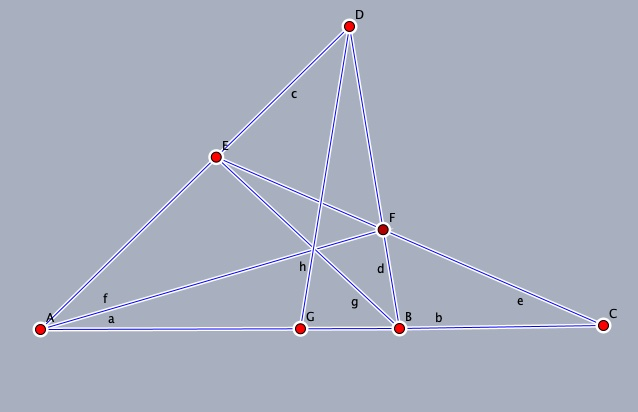
\includegraphics[width=30em]{CompleteQuad3.png} 
   \end{center}
     \protect \caption{A complete quadrilateral, consisting of the four points $A, B, C, D$ and the three lines joining them in pairs}
      \label{figCompleteQuad}
     \end{figure}
\end{center}

\bigskip 
\fix{Note to Editor: In Figure \ref{figCompleteQuad} please relabel the 7 points $A, B, C, D, E, F, G$ as $A, B, E, F, D, C, H$; remove the label $G$; label the point where the lines $AC$ and $BD$ cross (on the new labels) as $G$; delete the lower case letters that label the edges.}




The  \emph{Brouillon Project} is fiercely unreadable.\footnote{Happily, it has been the subject of sequence of detailed analyses in recent papers by Marie  Anglade and Jean-Yves Briend; see (Anglade and Briend 2022) and the references to their earlier papers cited there.} It was also lost for a long time and known only through commentaries by later authors until Michel Chasles found a handwritten copy made by Philippe de la Hire in 1845.\footnote{The only known copy of the original \emph{Brouillon project} turned up in 1950.} In particular, de la Hire, a generation after Desargues, wrote some much more readable, and longer, works in Desargues's spirit, illuminating the role of cross-ratio in the theory of tangents that came close to a theory of duality. Desargues's famous theorem on two triangles in perspective was published separately in (Bosse 1648).

The best attention Desargues's little book got was from his younger contemporary Blaise Pascal, who evidently produced a virtually complete theory of conics around what he called the ``mystical hexagram''. Unhappily, much of it is lost, and known to us only from some notes on it made by Leibniz, but the idea is that while there is always a conic through five points something happens if you want a conic through six points: we call it Pascal's theorem. Then, if you let the sixth point collapse onto one of the other five you get a tangent to the conic through those five points. One way or another all the key properties of conics are wrapped up in this idea, or so Pascal seems to have shown, and much of the early 19th century work in France can be seen as attempts to recover such a theory. It includes such topics as duality, in the form of the pole and polar relationship with respect to a conic (see Figure \ref{figpolepolar}).\footnote{For a thorough analysis of Pascal's work and its context, see (Del Centina 2020).} 


\fix{Note to Editor: In Figure \ref{figpolepolar} please delete the points $A, C, E$; relabel the points $B, D$ as $A, B$; make sure the lines through $A$ and $B$ that are claimed to be tangents really are, and label their point of intersection $P$.}
\bigskip
\begin{center}
    \begin{figure}
   \begin{center}  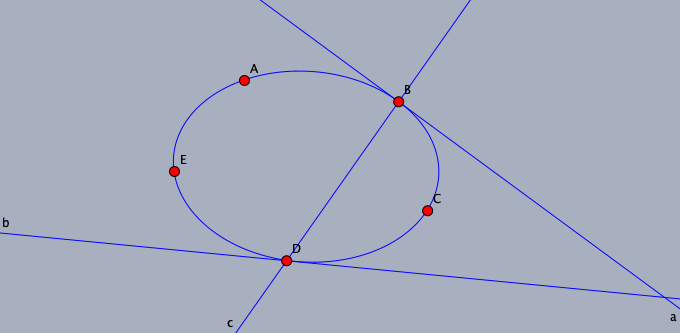
\includegraphics[width=30em]{poleandpolar.png} 
   \end{center}
     \protect \caption{The tangents from a point $P$ outside the conic touch it at $A$ and $B$; the line $AB$ is the \emph{polar} of $P$ and $P$ is the \emph{pole} of the line $AB$. The construction can be extended to points inside the conic.}
      \label{figpolepolar}
     \end{figure}
\end{center}

\bigskip 


Thereafter, truly projective geometry languished for much of the 18th century, despite some insightful contributions by Newton that we shall mention below (see p. ~\pageref{Newtonconics}) and a few others. Its revival is conventionally dated from the early work of Gaspard Monge, who as a young man seeking a job in the French army was  interested in how to depict three dimensions on two. He devised a method of plan and elevation (projections onto a horizontal and a vertical plane) that he could couple to some simple algebra in a way that was easy to use; as a result he was offered a job at the military Academy in M\'ezi\`eres and his discovery made a military secret. During the French Revolution, Monge was influential in setting up the \'Ecole Polytechnique, where he was an inspiring teacher of geometry, and this did much to revive the subject. 

Among those so inspired there was Jean Victor Poncelet, who promoted a much more general theory of transformations with a view to unifying the theory of conics that he began to develop while a prisoner-of-war in Saratov during Napoleon's disastrous invasion of Russia. His \emph{Trait\'e des Propri\'et\'es Projectives des Figures} (1822) is a visionary textbook that relies on some rather mysterious arguments about ideal points of intersection (Cauchy, who reviewed the book, urged that they be regarded as points with complex coordinates; Poncelet never agreed). As a result, some of the transformations it invokes necessarily require complex coordinates. The most famous result in the book is Poncelet's closure theorem, which has continued to attract attention to this day, but it is also notable for many other theorems involving pairs of conics.


In the 1820s, Poncelet had a dispute with Joseph Diaz Gergonne, the editor of the only journal at the time entirely devoted to mathematics, about what duality in the plane actually is.\footnote{Gergonne's journal was called the \emph{Annales de Math\'ematiques Pures at Appliqu\'ees}. It ran from 1810 to 1832, and  it was succeeded in by Liouville's \emph{Journal de Math\'ematiques Pures at Appliqu\'ees} in 1836. Crelle's \emph{Journal f\"ur die reine und angewandte Mathematik} was founded in 1826.}
Poncelet always saw it as pole and polar with respect to a conic, Gergonne saw it as a new and fundamental feature of projective geometry.\footnote{See (Gergonne 1826).} This led into confusion when applying it to curves of degree three or more, a matter that began to be sorted out only with Pl\"ucker's work, as we shall see below.


Another mathematician who was inspired by Monge was the Frenchman Michel Chasles, who used the projective invariance of the cross-ratio of four points to eliminate much of the weirdness of Poncelet's ideas. Independently, Jakob Steiner did very similar work in Germany. He can be credited with the first truly projective definition of a conic section. Even so, there remained an irritating feature of cross-ratio: it was given as a function of four lengths, but length is a property of Euclidean geometry, not projective geometry.  If projective geometry is to be regarded as more fundamental than Euclidean geometry, because it rests on fewer assumptions or axioms, then the intrusion of Euclidean length in the definition of cross-ratio is at the very least unfortunate. Nor can one easily speak of there being a concept of projective space in the 1820s; rather, much of geometry at this time was about figures in the plane subject to a variety of projective transformations. The first truly foundational work on real and complex projective geometry that avoided deriving it from Euclidean geometry was the achievement of von Staudt in his \emph{Geometrie der Lage} (1847), in a long and difficult work that influenced Felix Klein when he succeeded von Staudt as a Professor at Erlangen twenty-five years later. 

All in all, a surprising amount of work was done on the theory of conic sections  at the start of the 19th century, and before it is dismissed as arcane it should be stressed that the subject was a proving ground for the development of projective geometry. Two approaches stand out: the search for entirely  general methods that would treat all non-degenerate conics on a par; and the emergence of the property of duality. Matters are complicated by the existence of two separate traditions, usually called the synthetic and the analytic, supposedly divided into classical geometric methods and more algebraic ones that introduce coordinates. 
Recent historical work suggests that it was all a bit murky, and algebraic methods were also often used in synthetic geometry.\footnote{See (Lorenat 2016).} Several things promoted the use of synthetic methods. They can be elegant when algebraic methods are blunt; they correspond to the visual form of the conics; they provide a language for describing what is apparent or to be found in a problem. Against them is the obstinate fact that algebra is more general: it does not care if some quantities become negative, but what is a negative length? Once ways round that were found (by Poncelet and then Chasles) the way was open to a truly systematic synthetic theory of conics.   

How then did this change, and purely synthetic projective geometry begin to wane? Very few of the original protagonists disdained algebra outright, and as the (projective) theory of conics reached completion in the 1820s and established its fundamental character, being more general than metrical Euclidean geometry, it also had its baroque aspects. But worse, it did not generalise at all readily  to the study of curves of higher degree. For that, as even Newton had recognised, a hefty dose of algebra was required.







\section{Curves of higher degree from the 17th to the early 19th century} A common way to think of curves in antiquity was pointwise: some length depends in a given way on some other length. Accordingly, at least in principle, if you know the independent length
(the ordinate, or $x$ coordinate) you know the dependent length (the abscissa, or $y$ coordinate).  

By Descartes' time there was already some sophisticated algebra expressed in a formalism that hadn't quite shaken off   the Greek insistence on seeing everything as geometrical magnitudes: lengths, areas, volumes, and, well, what exactly? The French mathematician Fran\c{c}ois Vi\`ete in his \emph{Isagoge} boldly spoke of magnitudes having the dimensions of side, square, cube, square-square, square-cube and so on.\footnote{See his collected works, (Vi\'ete 1646).} It was possible to write polynomial equations in this language, as Vi\`ete did in the early 1600s. First Fermat in 1636, and then much more boldly Descartes in 1637, realised that you could extend the language to two variables and so describe curves in the plane.



\bigskip
\begin{center}
    \begin{figure}
   \begin{center}  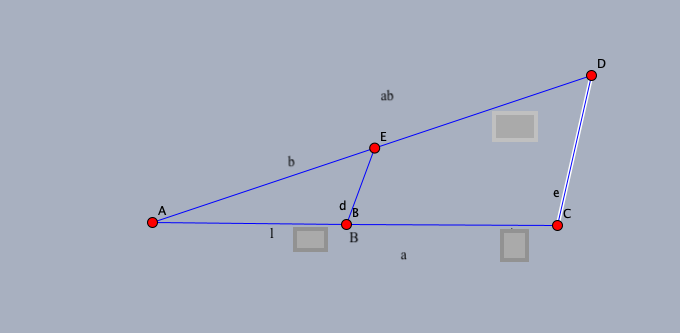
\includegraphics[width=30em]{Multiplication.png} 
   \end{center}
     \protect \caption{If $AB$ is of length 1, $AC$ of length $a$, $AE$ of length $b$, and $BE$ and $CE$ are parallel then AD is of length $ab.$}
      \label{figmultiplication}
     \end{figure}
\end{center}

\bigskip 

\fix{Note to Editor: In Figure \ref{figmultiplication} please move the lower case letters in that denote lengths to better positions, and eliminate the shaded rectangles.}

Descartes's first achievement in his \emph{La G\'eom\'etrie} (1637) was to eliminate the dimensional aspect. A simple use of similar triangles allowed him to show that the product of two lengths could be seen as another length (not an area) so all geometrical quantities could be regarded as one-dimensional and the idea of dimension quietly dropped (see Figure \ref{figmultiplication}). He also replaced Vi\`ete's cumbersome algebra, which was written in capital letters with verbal abbreviations for the algebraic operations, with something much more like   what we use today.  He wrote $x$ and $y$ for the key variables (not $A$ and $E$ in the manner of Vi\`ete). Descartes was clear that he was using coordinates, although his $x$ and $y$ coordinates could have oblique axes.


Then came the real work. Almost all mathematical problems in his day were expressed in the language of geometry, except for some problems we would call diophantine and were implicitly about integers and rational numbers. Accordingly, the answer had to be expressed geometrically. Descartes's idea was to give letters to all the lengths involved in a problem, use the statement of the problem to express relationships between the letters, and reduce the equations to a single equation. Then solve the equation and express the answer again in geometrical terms.  

 In this way he solved the famous Pappus problem (see Figure \ref{figPappusproblem}): given four lines and four angles (nothing is lost if we take these angles to be right angles), find the locus of points $P$ such that the product of the distances of $P$ from the first two lines is proportional to the product of the distances of $P$ from the last two lines. As he showed, and Pappus had known, the answer is a conic section, but  Descartes went further and claimed that in this way he could solve the Pappus problem for any number of lines. 
 
 \bigskip
\begin{center}
    \begin{figure}
   \begin{center}  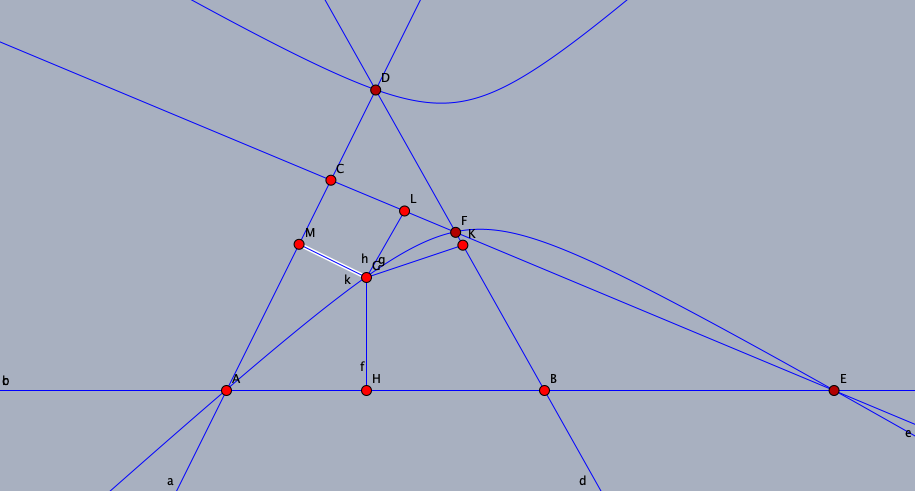
\includegraphics[width=30em]{Pappusproblem.png} 
   \end{center}
     \protect \caption{The Pappus problem: the product of the distances of $P$ from the lines $AB$ and $BC$ is proportional to the product of the distances of $P$ from the lines $CD$ and $DA$}
      \label{figPappusproblem}
     \end{figure}
\end{center}

\bigskip 

\fix{Note to Editor: in Figure \ref{figPappusproblem} please relabel $F$ as $C$, $C$  as $D$, and $G$ as $P$; remove the lower case letters; label the point in the middle $P$, and make sure that the four lines out of $P$ meet the four lines at right angles.}

This was to infuriate Newton, who showed that Greek methods were indeed adequate to the original Pappus problem. The background here is that Newton was also engaged in demolishing Descartes's theory of planetary motion in favour of his own, which led him into the theory of conic sections and to pose and solve the problem of finding the conic (or conics) through $n$ points and tangent to $5-n$ lines, which he did in Book I, Section 5 of his \emph{Principia Mathematica}.~\label{Newtonconics}

It can be argued that the theory of specifically algebraic curves has its origin in Descartes's method for finding normals to a curve at a point, which  involved considering all the circles through the given point and imposing the condition that the equation for the circle be such that it passes twice through the given point; this circle has its centre on the normal to the curve. On the basis of three examples, he claimed that the method always worked  if the curve had an algebraic equation, and he described a system of linkages (sliding rulers) that he said could be adapted to draw any such curve. Curves like the cycloid that were patently not algebraic he sought to exclude from geometry --- this exclusion was something else that annoyed Newton.

In the 1660s and 1670s, but only published  the 1690s and again in 1704 as an Appendix to his \emph{Opticks} Newton worked on a classification of cubic curves. He claimed that there were 72 distinct types which could be derived by simplifying the general equation using what we would call affine or linear transformations, although at one point he used a simple birational transformation. For some reason, in writing up his work for publication he omitted four of the possible cubics, and they were speedily found by various other mathematicians.  Newton also made the striking remark that this collapses to five types if projective transformations are allowed.\footnote{``The five divergent parabolas, by their shadows, generate all other curves of the second genus [i.e. cubic curves].'' See (Newton  1704) and Talbot (1860, p. 25).}





A plane cubic curve is defined by an equation involving ten coefficients, or more precisely by the nine ratios between the coefficients, which suggests that it should be determined by nine points in the plane because their coordinates provide nine equations that should determine these nine ratios.  Moreover, it seemed to mathematicians in the early 18th century that any set of nine points and therefore any set of nine equations in the nine unknowns should have a unique solution --- there was no theory of linear equations at the time ---  and as a result even the best mathematicians got into difficulties. For example, the Scottish mathematician Colin MacLaurin  knew in 1720 that there were problems with the idea that nine points in the plane should determine a cubic: any two cubics will meet in nine points, and so these nine points do not determine a unique cubic, and indeed there will be infinitely many cubics through these nine points.\footnote{MacLaurin also knew that a general cubic curve has nine flexes, and the line joining any two passes through a third.}  MacLaurin did not, however, know how to solve this puzzle. His observation was conveyed to Euler by his friend the Swiss mathematician Gabriel Cramer  in 1744. This apparent contradiction with the claim that nine points in the plane always determine a unique cubic became known as Cramer's paradox.  Part of the confusion at the time was a lack of insight into systems of linear equations, and part was the lack of understanding about what are the implications of configurations that do not determine a unique curve. 

More interestingly, when Cramer addressed the problem in his book (1750, Chapter 3) he suggested that if the $\ha n(n+3)$ points needed to determine a curve of degree $n$ contain $tn$ points common to a curve of degree $t < n$ then the curve through the  $\ha (n+1)(n+2)$ points breaks up into two or more curves, one of which passes through the $tn$ points. We note that Cramer considered only irreducible curves: a circle and a line, for example, would be considered as two curves, not one.\footnote{Curves were taken to be irreducible even in Salmon's book \emph{Higher Plane Curves} (1852).} 


The (incorrect) claim about cubic curves, and more generally the analogous claim for curves of degree $n$, that they are determined by $\ha n(n+3)$ general points, was repeated  by  Euler  in the second volume of his \emph{Introductio} (1748, \S\,81). He then wrote a paper (Euler 1750) in which he first spelled out the problem. It is a general proposition, he said, that $k$ linear equations in $k$ unknowns have a unique solution. Accordingly, 9 points in the plane will determine a unique cubic curve. But nine points common to two cubics plainly do not determine a unique cubic curve. To resolve this apparent contradiction, as he called it, he began with  three equations in three unknowns and showed by example that there will not be a unique solution if one of these equations is contained in (that is, is a consequence of) the others. He drew the same conclusion about four linear equation in four unknowns, and stated more generally that there will not be a unique solution to a system of $n$ equations in $n$ unknowns if one or more are contained in all the others. 

He then turned to the geometrical implications. In the case of conics, he showed that the containment condition corresponds to the case when four, or all five, of five given points lie on a line.  For cubics, he remarked that one easily understands that not just one, but two or more of the nine equations specified by nine points may be contained in the others, and to obtain a unique cubic it will be necessary to specify that the curve passes through one or more additional points.  However, he said, it was very difficult to see what the consequences were when this is the case, because there were so many points and coefficients that things become too complicated, although it was possible to draw conclusions in simple cases. For example, if the nine equations arise in part from four points lying on a line then the remaining five equations must determine a conic, which might itself consist of two lines. Euler concluded his paper with a few remarks about curves of higher degree.


The idea that algebraic curves of degrees $k$ and $m$ in the plane should meet in $km$ points was something of a folklore result in the early 18th century, but it travelled without a proof for many years. Euler discussed it in the second volume of his  \emph{Introductio} (1748, Ch. 19) and noted that even in simple cases  for the counting to work one would have to take care of multiple points (such as tangents),  points `at infinity' (consider a parabola and a line parallel to its axis), and allow the  coordinates of intersection points to be complex (consider the intersection of two circles). The first person to find a persuasive way of tackling the problem was \'Etienne B\'ezout, who lived from 1739 to 1783, and made his living teaching mathematics at the French military and naval academies. He published the theorem that bears his name in a book of 1779; it is based on his theory of the resultant of two polynomial equations that he developed in a paper of 1764. His proof of the theorem is gappy and intuitive by any standards, but so much better than what had been done before that his immediate successors were willing to give him real credit for doing as much as he did. His results inspired later work by Cauchy and Sylvester.

To state  B\'ezout's theorem in general requires a notion of the multiplicity of an intersection of two plane curves without common components. Such a notion was developed by Max Noether, and refined by Macaulay. A modern proof would invoke Noether's Fundamental Theorem --- see p. \pageref{Noether'sFT} --- and a computation of the Hilbert polynomial. This is a story that  has been pursued, with successive new generalisations, right up to the present day. 


As this work suggests, throughout the 18th century mathematicians had become more and more comfortable with the idea of complex numbers in algebra, and with the idea of proving that a polynomial of degree $n$ has $n$ roots, possibly with repetitions (the so-called fundamental theorem of algebra).\footnote{For a history of attempts on this theorem, see (Gilain 1991).} Euler's attitude to complex numbers was that there was nothing to explain. Although they cannot be ordered, expressions of the form $a+bi$  behave arithmetically like numbers, so they can reasonably be considered numbers  and ``are usually called \emph{imaginary quantities}, because they exist merely in the imagination.''\footnote{See Euler, \emph{Algebra} \S\, 143, p. 43. Euler here rejected the idea that ultimately mathematical quantities must be exhibited in nature: three sheep, a length of $\sqrt{2}$, and so on.} Cauchy's view later was more explicit and very close to regarding  the field of complex numbers as $\RR [x]/(x^2 + 1)$. This works for finding a proof of the fundamental theorem of algebra, which he gave a proof of in his (1817a, b), but was not productive in contexts involving contour integration. 

Credit for the first rigorous proof of the fundamental theorem is often given to Gauss for his paper (1799), although he did base his argument on the claim that an algebraic curve that enters a bounded region of the plane also leaves it,  which is surely no easier to prove.  Gauss went on to give three more proofs of the theorem, and soon any doubts about the algebraic nature of complex numbers were resolved.\footnote{William Rowan Hamilton published his rigorous theory of ordered pairs of real numbers in his (1837).} Abel and Jacobi, in their work  on elliptic functions, took a formal, non-geometrical attitude to complex numbers.  Both men were algebraists at heart -- formidable algebraists -- and the exact nature the plane of complex numbers did not really interest them. 

All things considered, however, progress in the study of cubic, quartic, and higher degree curves in the 18th century was piecemeal and slight, and the sheer enormity of the equations involved seems to have baffled even Euler. New methods for handling such curves would have to be found, such as came in with Julius Pl\"ucker in the 1820s. His key idea was to study families of curves, using the symbolic notation devised by Gergonne.\footnote{See  (Gergonne 1826--1827), (Pl\"ucker 1835) and (Pl\"ucker 1839).} If $S_1$ and $S_2$ stand for the equations of two curves of the same degree, then $S_1 + \lambda S_2$ is the equation of another curve of that kind. This may be the first occurrence of the idea of a linear series, with which this book is much concerned. Using this idea allowed Pl\"ucker to pull out geometrical properties of cubic and quartic plane curves while avoiding the algebraic complexities that had defeated Euler.  

Pl\"ucker also resolved the paradox about dual curves in the theory of plane curves in his (1834) that had stumped Gergonne and Poncelet. The paradox arises because the dual of a smooth curve of degree $d$ has degree $d(d-1)$
so the dual of the dual ``ought'' to have degree $d(d-1)(d(d-1)-1)$. However, the dual of the dual is the original curve.  
Pl\"ucker's response, which would strike us today as at best heuristic, was that any line through a double point, say, is counted in this way as a tangent, and this throws the count of genuine tangents off. More precisely, he  showed that each node on a curve reduces the degree of the dual curve by 2, and each cusp reduces it by 3. Consequently, he claimed that  a curve of degree $d$ with $\delta$ double points and $\kappa$ cusps has a dual curve  of degree $d(d-1) -  2\delta - 3\kappa.$ 




Pl\"ucker also showed in his (1839, 207--227) that the nodes of $C^{*}$  corresponded to the bitangents of $C$, while the cusps of $C^{*}$ corresponded to the flexes of $C$, and vice versa. To see how he resolved the duality paradox, consider  the case of a non-singular cubic curve. It has no nodes, cusps, or bitangents, and as yet an indeterminate number, $j$ of flexes. Its dual has degree 6 and $j$ cusps. The dual of the dual curve therefore has degree $6.5 - 3j$, which will equal 3 if $j = 9.$ As we saw, the result that a non-degenerate cubic curve has nine flexes had been known since MacLaurin. For curves of higher degree, it is necessary to consider a curve of degree $n$ that has $\delta$ double points, $\kappa$ cusps, $\tau$ bitangents, and $\iota$ inflections. Suppose that its dual has degree $n'$. Pl\"ucker argued that
\[n' = n(n-1) - 2\delta - 3 \kappa,\]
\[{\rm and}\; \iota = 3n(n-2) - 6\delta - 8\kappa,\]
with another formula for $\tau$, along with the corresponding formula for the dual curve and its inflection points and bitangents.

The number $\iota$ is most easily found using an argument due to Hesse, who showed  in his (1844)  that the set of flexes $\Gamma\subset G$ on a curve $G$ of degree $d$ with equation $F(x, y, z) = 0$ could be characterized as the intersection of $G$  with the curve $D$ defined by the vanishing of the \emph{Hessian determinant}:
$$
H = \det \begin{pmatrix}
 \partial^{2}F/\partial x^{2} &\partial^{2}F/\partial x\partial y &\partial^{2}F/\partial x\partial z \\
\partial^{2}F/\partial x\partial y  &\partial^{2}F/\partial y^{2} &\partial^{2}F/\partial y\partial z \\
\partial^{2}F/\partial x\partial z &\partial^{2}F/\partial y\partial z &\partial^{2}F/\partial z^{2} 
\end{pmatrix}.
$$
Since the entries of this matrix have degree $n-2$, the degree of $H$ is $3(n-2).$ For general $F$ the curves $G$ and $D$ meet transversely, so B\'ezout's Theorem shows that a general curve of degree $m$ has exactly $\iota = 3n(n-2)$ flexes.\footnote{This result was first proved in a different way in (Pl\"ucker 1835, 264), as Hesse acknowledged.}

The most famous case Pl\"ucker established in  his book (1839, 247),  concerns   a nonsingular plane curve $C$ of degree $n=4$  (no nodes, cusps, or other singular points) having $\tau$ bitangents and $\iota$ flexes.   Its dual curve has degree 12 and will have $\tau$ double points and $\iota$ cusps, and the dual of the dual will have degree 
$12\cdot 11 - 2\tau - 3h  = 4.$ 
Hesse's theorem shows that $h = 24$ (Pl\"ucker  had an ad hoc argument to the same effect)  and so $\tau = 28$,  and we  see that $C$ has exactly 28 bitangents. Pl\"ucker showed that they can all be real (see Figure \ref{fig28bitangents}).

In 1849, Pl\"ucker gave up mathematics for physics, particularly the study of cathode rays; he was awarded the Royal Society of London's Copley medal (its highest honour) for this work in 1866. It is sometimes said that he gave up geometry because he tired of the criticisms of Steiner, who had a secure position in Berlin and influenced the decisions of the \emph{Journal f\"ur Mathematik}, and only returned to geometry after Steiner died in 1863. Now he took up  the field of line geometry, which he transformed into a new branch of the subject. 

\bigskip

\begin{center}
    \begin{figure}
   \begin{center}  \includegraphics[width=15em]{28bitangents} 
   \end{center}
     \protect \caption{\, Pl\"ucker's quartic curve has 28 bitangents, from (Pl\"ucker 1839)}
      \label{fig28bitangents}
     \end{figure}
\end{center}
\bigskip

Pl\"ucker's formulae work well for curves of degrees 3 and 4,  but not so well thereafter because other types of singularity can appear.   He listed all the solutions he could find to the equations that bear his name up to curves of degree 10, but he did not discuss the kinds of singularities a curve may have that are not of the type he had considered.\footnote{See (Pl\"ucker 1839, 214).}  Progress was only made with a paper by Cayley (1866), who drew on Puiseux's paper (1850) that analysed  how curves are ramified at a singular point,  showed how the branches are permuted in cycles, and how this is captured by the local power series expansions, which begin with fractional indices.\footnote{Cayley's paper was corrected by Otto Stolz in his (1875), who found that the conclusions were correct but the proof ``as he [Cayley] himself remarks'', was not quite complete.}

Puiseux was one of a number of mathematicians in the circle around Cauchy. Cauchy had spent the 1830s and early 1840s following the Bourbon Court around Europe from a strange belief that the oath of allegiance he had sworn to the crown on becoming a professor compelled him to do so. As a result, by 1850 few people knew the work he had done in those years, and even he seems to have forgotten what he had done in complex variable theory back in the 1820s, which included a version of what we call the Cauchy integral theorem restricted to rectangular contours. Only on his return to Paris did he begin to think much more geometrically; previously his attitude to a many-valued `function' was to cut the plane and study just a branch of it on what remains. His understanding of branch points was quite limited, and this left space for Puiseux to study integrals on arbitrary contours   and what happens to integrals taken around branch points. 

\section{The birth of projective space}
When did projective space come in, regarded as something more rigorous than Euclidean space with a ``line at infinity''?\footnote{For an interesting  set of essays analysing what projective space might be and how it came about, including an extensive analysis by J.-P. Friedelmeyer of the work of Poncelet, see (L. Biosemat-Martagon 2010), and the discussion in del Centina (to appear).}
 This might simply be a suitable set of coordinates. Pl\"ucker used coordinates for the plane with a line at infinity in his (1830) with a view to enabling homogeneous equations to correspond to curves; in this system the coordinates $(p, q, r)$ denote the signed distances of a point from the three sides of a triangle of reference. However, in his study of curves (1835) he would first discuss them in  the plane, and then as they went off to infinity; he didn't say that the line at infinity could be mapped by a projective transformation into the finite part of the plane.  The way forward was indicated by M\"obius, who introduced barycentric coordinates in his (1827). Pick three points forming a triangle, say $ABC$, and attach weights, positive, zero, or negative (not all zero) to these points. The barycentre or centre of gravity of these three weighted points is a point $P$ which can be said to have those three weights (or, better, their ratios) as its barycentric coordinates. If you put the points $A, B, C$ at, say,  $(0, 0), (1, 0), (0, 1)$ you get an easy way to relate points in what could be called the Cartesian and barycentric coordinate planes. The big plus is that the line at infinity, which is invisible in Cartesian coordinates, is a perfectly sensible line in barycentric coordinates. In this system, a line has an equation of the form $ax+by+cz=0,$ and by treating $a, b, c$ as the coordinates of the line M\"obius obtained a simple theory of conics and duality in the plane. (He also showed that there are dualities in $P^3$ that are not pole-polar dualities.)

If you drop the talk about weights, and keep the idea that barycentric coordinates are best thought of as ratios of three numbers, you have projective coordinates; this was one of the contributions of Otto Hesse in the 1840s.\footnote{See, for example, his (1844).}
Mathematicians were still reluctant, however, to decide if this space was $\PP_\RR^2$ or, less likely, $\PP_\CC^2$. 
 


Mathematicians found it  hard to accept complex coordinates,  even though Pl\"ucker used the term `imaginary'  (as in `imaginary' points, `imaginary' straight lines, `imaginary' tangents) over two hundred times in his   (1828--1831).\footnote{Del Centina, forthcoming.} He employed the term confidently in his (1839) when, for example, he discussed how many of the 28 bitangents to a quartic curve can be real. In fact, the whole question of a complex space was obscure for a long time. As late as 1878 Cayley could write about complex curves as sets of points in $\CC \times \CC$ and remark ``I was under the impression that the theory was a known one; but I have not found it set out anywhere in detail.''\footnote{See (Cayley 1878, 32).} For quite some time attention was fixed on real curves in the real plane, which could conveniently sprout points with complex coordinates when they intersected other curves. This unstable situation could not last, but how it was to be swept away was not clear to mathematicians initially. 


\section{Riemann's theory of algebraic curves and its reception}
It was, however, entirely clear to Riemann. The crucial issue in defining complex-valued functions of a complex variable, where a complex variable can be taken as an expression of the form $x+ iy$, is defining what it is for such a function to be something more particular than a mapping from $\RR^2$ to $\RR^2$, and this comes down to defining what it is for such a function to be differentiable as a function of a complex variable. As is well-known, Riemann solved this problem in the opening pages of his inaugural dissertation  (1851) by identifying -- much more clearly than Cauchy -- the role of what we call the Cauchy--Riemann equations. He proceeded to give a thoroughly geometric theory of complex functions, which he extended in his great paper on Abelian functions (1857). There he developed a strikingly topological account, which classified orientable, boundaryless surfaces by the number, $2p+1$, of cuts needs to disconnect them. He called this number the order of connectivity of the surface, when $p=0$ he called the surface simply connected. The theory is too complicated to be described fully here, but briefly, he showed that  the dimension of the space of ``everywhere finite'' differential forms on such a surface is $p$, and the integral of each such 
differential gives rise to a many-valued function, which can be expressed in the form $f(z, w) = 0$, where $z$ and $w$ are complex variables. He also deduced the Riemann inequality in this form (1857, \S\, 5):  the number of arbitrary constants in a function $w$ that has $m$ first-order poles on a surface of order of connectivity $2p+1$ is $m- p + 1$ when $m \geq p + 1$. He gave a more detailed account that involves special cases that were interpreted by his student Roch to give us the Riemann--Roch theorem. 

Riemann's health started to decline in the early 1860s, and he  died in Italy in July 1866. By then, Rudolf Clebsch had decided to develop Riemann's ideas and to try to persuade people around him to take up the cause. In his (1864) he  applied the theory of Abelian functions to the study of plane algebraic curves. Here he used coordinates that belonged  either to $\CC^2$ or $\PP_\CC^2$ and  passed easily between them as required, so it would seem that he and the people he influenced had become comfortable with complex projective space in all but name.

                                                                                                                                                                                                                                                                                                                                                                                                                                                                                                                                                                                                                                                                                                                                                                                                                                                                                                                                                                                                                                                                                                           
In his papers (1865a, 43) and (1865b, 98) Clebsch sorted curves into different genera according to the value of the number $p$ associated to them, but he did not speak of the genus of a curve.\footnote{See (L\^e 2020), who suggests that Felix Klein was the first to do so.} If we allow ourselves to do so, we may say that Clebsch defined the genus of a plane algebraic curve with $\delta$ double points as\footnote{See (Clebsch 1864, 192).} 
 \[p = \ha (n-1)(n-2) - \delta.\]
In his (1865b) and his book with Paul Gordan (1866) he extended this to encompass curves with 
$\kappa$ cusps, so $p= \ha (n-1)(n-2) - \delta - \kappa.$ This tells us incidentally that no singular points more complicated than those considered by Pl\"ucker in the late 1830s had been looked at. Clebsch's formula relied on being able to count the number of constants in an integral of an everywhere finite differential correctly, a result that requires the  completeness of the adjoint series. Clebsch and Gordan, in their book (1866, Chapter 3) offered a proof that the genus of a plane algebraic curve is invariant under a birational transformation, but it was valid only for the case of a curve with simple cusps and double points. 


Clebsch became   Riemann's successor in G\"ottingen in 1868, but  he died of diphtheria in 1872 at the age of 39. His plans for the study of algebraic geometry now devolved upon Alexander Brill and Max Noether, with whose theory, modernised and made rigorous,  this book is in part concerned.\footnote{A modern account of  much of the material described above can be found in (Brieskorn and Kn\"orrer 1986). (Coolidge 1940) remains a historically informative if not entirely rigorous account of many of these developments, more additional mathematical details are in (Coolidge 1931).}

Alexander Wilhelm Brill was born in Darmstadt in 1842.\footnote{See (Severi 1922),  and Brill's obituary (Finsterwalder 1936).} His  uncle was the mathematician Christian Wiener, an expert in descriptive geometry. He entered the University of Giessen intending to study architecture but his mathematical ability brought him to the attention of Clebsch, who was then at Giessen and who encouraged him to go  to Berlin, where  Ernst Kummer,  Leopold Kronecker, and Karl Weierstrass taught. This broadened Brill's horizons considerably, but he returned to Giessen in 1867 to take his Habilitation  under Clebsch.

In Giessen, Brill met Max Noether. Noether had been born in Mannheim in 1844, but polio at the age of 14 left him paralysed in one leg and delayed his education. He had to be privately schooled, which gave him  broad literary and cultural interests. At university he  initially intended to study astronomy, but then he switched to mathematics, first at Heidelberg and then at Giessen and G\"ottingen in 1868 and 1869. He habilitated in Heidelberg in 1870 with a thesis on surfaces possessing a family of rational curves. In 1875 he became a Professor at Erlangen, where he remained until his death in 1921.\footnote{See his obituary (Brill 1923).} 


Noether  worked not only on plane algebraic curves, including the analysis of their singular points, but the geometry of algebraic surfaces,  algebraic curves in space, and Cremona transformations of the plane;  van der Waerden justly remarked that ``Algebraic geometry was created by Max Noether.''\footnote{See (Waerden 1971, 171) who immediately commented that the logical foundations are shaky.} 
He drew largely on the work of Pl\"ucker on algebraic curves and their singular points, and was less interested in the computational side of the theory that Clebsch had emphasised. As a result, his obituarists --- Guido Castelnuovo, Federigo Enriques, and Francesco Severi --- noted that Noether's work was inclined to be qualitatively valuable even though he may not have paid sufficient attention to ``contingent aspects of the formulae''.  However, they added that:\footnote{See (Castelnuovo, Enriques, and Severi 1925, 162)}
\begin{quote}
geometric intuition, which was always his guide, saved him from error, and the work, even if it was not perfect, and perhaps for that reason, was richly suggestive.
\end{quote}



Brill  chafed under the direction of  Richard Baltzer, who was Clebsch's successor at Giessen,  and moved to the new Polytechnic in Darmstadt in 1869, which was academically a step downwards. There, he did his work on the Cayley--Brill correspondence principle, and in 1875  he accepted Klein's offer of becoming a Professor at the Polytechnic in Munich, with responsibility for reforming high school education.  Brill found Klein's inventiveness hard to match, but he enjoyed getting to know some of the other mathematicians there, including Philipp Seidel and the young Alfred Pringsheim. Among his pupils were Walther Dyck, Isaak Bacharach, and Ferdinand Lindemann, who went on to produce the two-volume geometry textbook \emph{Vorlesungen \"uber Geometrie} (known as Clebsch--Lindemann) before achieving fame as the mathematician who proved that $\pi$ is transcendental.


\section{First ideas about the resolution of singular points}
In their work on algebraic curves, Brill and Noether found Riemann's use of the Dirichlet principle at the heart of his theory of complex analytic functions to be unsound, so they studied curves firmly in the complex plane $\CC^2$ or the complex projective plane $\PP_\CC^2.$ They were concerned to treat such curves in full generality, and this led them to confront the issue of arbitrary singularities of plane curves. Their preferred method was to argue that any curve with whatever singularities could be reduced to one of the same genus but having only double points by a sequence of Cremona transformations, and then to deal in detail with these simpler curves. It was clear from the formula for the genus of a plane curve that if the genus of the curve is not a triangular number then the curve will always have singular points, so the process of desingularising cannot always lead to a nonsingular curve.

Luigi Cremona had  outlined a general theory of transformations of the plane in his papers (1863) and (1865). He looked for geometrical transformations of the plane mapping a given figure one-to-one onto its image, and reciprocally; notably  transformations that map straight lines to curves of order $n$, for some $n.$ When $n=2$ (the case of quadratic transformations)  as he showed, almost all straight lines must have images that are conics passing through 3 fixed points.\footnote{Such examples had been studied before, Cremona  cited papers by Steiner, Magnus, and Schiaparelli, but for higher values of $n$, which Cremona analysed in his (1865), everything was new.}



Noether in his (1871a) was the first to appreciate that Cremona transformations could be used to simplify singular points.  He wrote a Cremona transformation of the plane algebraically as 
\[[x, y, z] \mapsto [x', y', z'] = [\phi (x, y, z), \psi (x, y, z),  \chi (x, y, z)], \]
where the functions $\phi, \psi$ and $\chi$ are homogeneous polynomials in $x, y$ and $z$ of the same degree. To simplify a singular point he used
transformations defined as above where $\phi, \psi$, and $\chi$ all vanish at the singular point.  In the affine plane this becomes
\[(x , y) \mapsto (x_1 , y_1) = \left(\frac{\varphi (x, y)}{\chi (x, y)}\;,  \frac{\psi (x, y)}{\chi (x, y)} \right),\]
where $\varphi$, $\psi$, and $\chi$ are polynomial functions that vanish at the singular point.  To see what this does, it is convenient to take the familiar example of 
the simplest  Cremona transformation, other than a projective transformation. It  is given algebraically by  the quadratic transformation 
\begin{equation}~\label{eq:qt1}
[x, y, z] \mapsto \left[\frac{1}{x}, \frac{1}{y}, \frac{1}{z}\right] = [yz, zx, xy]\end{equation}
The union of the lines $x=0,y=0,z=0$ is called the exceptional triangle, and the images of these lines are the points $[1, 0, 0], [0, 1, 0]$ and $[0, 0, 1]$ respectively.
The transformation is many-valued at these points, each of which is ``blown up'' into a line  but it is well-defined away from those three points and it is  one-to-one away from  the lines $x=0$, $y=0$, and $z = 0.$ 


Noether's argument that any plane algebraic curve can be reduced to one with only double points is sketchy at best. His use of Puiseux's work suggests that he appreciated that quadratic transformation might have to be used repeatedly to reduce a complicated singularity to a simpler one, but he did not  fully appreciate what happens to the rest of the curve at the points where it crosses the exceptional lines. In his more rigorous account  (1876),  he gave a better definition of a singular point, and tried to redefine the genus of a plane algebraic curve and prove its  invariance  under birational  transformations.\footnote{Noether also claimed  the remarkable theorem that every such Cremona transformation is a composition of quadratic transformations and projective transformations. See his (1871b), with a small correction in his (1873).} 


\section{The work of Brill and Noether}
Noether began, in his (1873), with the question of when  a plane curve $E$ with equation $H=0$ can be expressed in the form $H = AF+BG,$ where $F=0$ and $G=0$ are the equations of two curves $C$ and $D.$ He rightly pointed out that people hitherto had assumed that it was necessary and sufficient that the curve $E$  passes simply through the intersection points of the curves $C$ and $D$, but in fact this is insufficient when the curves $C$ and $D$ have singular points or intersections with multiple tangents. His own account, which was based on counting the number of independent equations imposed on $H=0$ by the equations $F=0$ and $G=0$, was a significant advance, but it too had flaws and he and other authors, notably Bertini, offered improvements. Eventually, Noether  offered this formulation of his  Fundamental Theorem\label{Noether'sFT}:\footnote{See (Noether 1887, 413).}
\begin{theorem}~\label{NFT1887}
$H(x, y)$ is representable in the form $AF + BG$ if and only if in some neighbourhood of each common point $(x_0, y_0)$ of $F=0$ and $G=0$ there are power series $a(x-x_0)$ and $b(x-x_0)$ in $\CC[y][[x]]$ whose coefficients are polynomials in $y$ of orders  $n-1$ and $m-1$ respectively, such that $H = aF + bG.$ 
\end{theorem}
Only in the monumental joint work with Brill (Brill and Noether 1894, 352) was it shown that in the plane case there is nothing more to be said, the local conditions are indeed sufficient even in the projective case.


Today we would say that Noether's Fundamental Theorem is true for two polynomials $F$ and $G$ because $F,G$ is a regular sequence  and so  the ideal they generate is, in later terminology due to Macaulay (1916), unmixed.\footnote{See (Eisenbud and Gray 2023) and (Eisenbud and Gray 2024) for a historical account of Macaulay's work.}


Brill and Noether recognised that the Riemann-Roch Theorem, was of  central importance to the theory of plane algebraic curves; indeed, they were the first to name it.\footnote{See (Brill and Noether 1874, \S\,5).}  Clebsch had studied what we would call holomorphic differential forms on a curve $C$  of degree $d$ in his (1864, 193)  by supposing that they are given by homogeneous polynomials of degree $d-3$ that vanish at the double points of the curve. 
By B\'ezout's Theorem, such an intersection also has degree $d(d-3) = 2p-2$, as it should. The dimension of the family of divisors cut out on $C$ in this way is the dimension of the projective space of forms of degree $d-3$ in $\CC[x_0,x_1,x_2]$, which is conveniently equal to $(d-1)(d-2)/2$. For this to be correct and account for all the canonical divisors, it has to be shown that every divisor $E$ on the curve $C$ that differs from an intersection $D\cap C$, where $D$ is the curve defined by the equation $G = 0$,  by the divisor of the restriction to $C$ of a rational function $P/Q$ (where $P, Q$ are forms of the same degree), is again of the form $D'\cap C$ for some curve $D'$. This is the content of Noether's Fundamental Theorem. His Fundamental Theorem is essential when it comes  to handling  sets of points cut out on a fixed curve $C$ by families of curves, counting the degree of an intersection of two curves at multiple points,  dividing an arbitrary intersection into two subsets, and delivering a satisfactory version of the Riemann-Roch Theorem. 












 

\section{Bibliography}
\small
\indent Anglade, M. and J.-Y. Briend 2022. Nombrils, bruslans, autrement foyerz; la g\'eom\'etrie en action dans le \emph{Brouillon project} de Girard Desargues, \emph{Archive for History of Exact Sciences}, 76, 173--206.
\newline\indent B\'ezout, E. 1764. Sur le degr\'e des \'equations r\'esultantes de l'\'evanouissment des inconnues, \emph{M\'emoires de l'Acad\'emie Royale des Sciences}, 288--338.
\newline\indent B\'ezout, E. 1779. \emph{Th\'eorie g\'en\'erale des \'equations alg\'ebriques}, Ph.-D. Pierres, Paris, 1779. English translation by Eric Feron, Princeton University Press, 2006.
\newline\indent  Biosemat-Martagon, L. 2010. \emph{El\'ements d'une biographie de l'Espace projectif}, Presses Universitaires de Nancy.
\newline\indent Bombelli, R. 1572 \emph{L'algebra}, Bologna.
\newline\indent Bosse, A.  1648. \emph{Maniere universelle de Mr. Desargues pour pratiquer la perspective, etc}, Paris.
\newline\indent Brieskorn, E. and  H. Kn\"orrer 1986. \emph{Plane Algebraic Curves} Birhh\"auser.
\newline\indent Brill, A. 1923. Max Noether, \emph{Jahrsbericht den Deutschen mathematiker Vereinigung} 32, 211--233.
\newline\indent Brill, A. and M. Noether  1874.  Ueber die algebraischen Functionen und ihre Anwendung in der Geometrie, \emph{Mathematische Annalen} 7, 269--310.
\newline\indent Brill A. and M. Noether 1894  Die Entwicklung der Theorie der algebraischen Functionen in alterer und neuerer Zeit, \emph{Jahrsbericht den Deutschen mathematiker Vereinigung} 3, 107--566.
\newline\indent Cardano, G. 1545  \emph{Artis Magnae sive de regulis algebraicis liber unus}, Nuremburg. 
\newline\indent Castelnuovo, G., F. Enriques, and F. Severi, 1925 Max Noether, \emph{Mathematische Annalen} 93, 161--181.
\newline\indent Cauchy, A.-L. 1817a. Sur les racines imaginaires des \'equations. \emph{Nouv. Bull. Soc. Philom.} 5--9, in  \emph{Oeuvres Compl\`etes} (2) 2, 210--216.
 \newline\indent Cauchy, A.-L. 1817b. Seconde note sur les racines imaginaires des\'equa\-tions. \emph{Nouv. Bull. Soc. Philom.} 161--164, in \emph{Oeuvres Compl\`etes} (2) 2, 217--222.
\newline\indent Cayley, A. 1866. On the higher singularities of a plane curve, \emph{Quarterly Journal of Pure and Applied Mathematics} 7, 212--223, in \emph{Collected Mathematical Papers} V, no. 374, 520--582.
\newline\indent   Cayley, A. 1878. On the geometrical representation of imaginary variables by a real correspondence of two planes, \emph{Proceedings of the  London Mathematical Society} 9, 31--39 in \emph{The Collected Mathematical Papers of Arthur Cayley} X, no. 689, 316--323.
\newline\indent Chasles, M. 1837.  \emph{Aper\c{c}u historique sur l'origine et le d\'eveloppement des m\'ethodes en g\'eom\'etrie}, Hayez, Bruxelles. 
\newline\indent Clebsch, R.F.A. 1864.  Ueber die Anwendung der Abelschen Functionen in der Geometrie, \emph{Journal f\"ur die reine und angewandte Mathematik}  63, 189--243.
\newline\indent Clebsch, R.F.A. 1865a. Ueber die diejenigen ebenen Curven, deren Coordinaten rationale Functionen eines Parameters sind \emph{Journal f\"ur die reine und angewandte Mathematik} 64, 43--65.
\newline\indent Clebsch, R.F.A. 1865b. Ueber die Singularit\"aten algebraischer Curven, \emph{Journal f\"ur die reine und angewandte Mathematik} 64, 98--100.
\newline\indent Clebsch, A. and P. Gordan 1866. \emph{Theorie der Abelschen Functionen}, Teubner, Leipzig.
\newline\indent Cohen, M.R. and Drabkin, I.E. 1948. \emph{A Source Book in Greek Science}, Harvard University Press.
\newline\indent Coolidge, J.L.  1931 \emph{A Treatise on Algebraic Plane Curves} Oxford U.P. , Dover reprint 2004.
\newline\indent Coolidge, J.L.  1940  \emph{A history of geometrical methods}, Oxford U.P., Dover reprint 2003.
\newline\indent Cramer, G. 1750. \emph{Introduction \`a l'analyse des lignes courbes alg\'ebriques}. Fr\`eres Cramer et Cl. Philibert, Geneva.
\newline\indent Del Centina, A. 2020 Pascal's Mystic Hexagram, and a conjectural restoration of his lost Treatise on Conic Sections. \emph{Archive for History of Exact Sciences} 74.5, 469--521.
\newline\indent Desargues G. 1639. \emph{Brouillon project d'une atteinte aux evenements des rencontres du Cone avec un Plane}, Paris.  J.V. Field  and J.J. Gray (eds. and transl.)\emph{The geometrical work of Girard Desargues}, 1987, Springer, New York.
\newline\indent Descartes, R. 1637 \emph{La G\'eom\'etrie} in \emph{Discours de la M\'ethode, etc.} Leyden, English transl. \emph{The Geometry of Ren\'e Descartes}, D.E. Smith and M.L. Latham, Open Court 1925, Dover reprint 1954.
\newline\indent Eisenbud, D.E. and J.J. Gray, 2023 F.S. Macaulay: From plane curves to Gorenstein rings, \emph{Bulletin (new series) of the American Mathematical Society} 
60.3,  371?406, https://doi.org/10.1090/bull/1787
\newline\indent Eisenbud, D.E. and J.J. Gray, to appear \emph{F. S. Macaulay: from plane geometry to modern commutative algebra}
\newline\indent  Euler, L. 1748. \emph{Introductio in Analysin Infinitorum}, two vols., \emph{Opera Omnia} (1) Vols. 8 and 9, transl. \emph{Introduction to Analysis of the Infinite}, Book I,  Springer, 1988, Book II, Springer, 1990 (E101, E102).
\newline\indent  Euler, L. 1750.  Sur un contradiction apparente dans la doctrine des lignes courbes. \emph{M\'emoires de l'Acad\'emie des Sciences de Berlin} 4, 1750, 219--233, in  \emph{Opera Omnia} (1)   26, 33--45 (E147).
\newline\indent Euler, L. 1770. \emph{Vollst\"andige Einleitung zur Algebra} in \emph{Opera Omnia} (1) 1,  transl. \emph{Elements of Algebra}, Rev. J. Hewlett, London, 1840, repr.  Springer, 1972 (E387).
\newline\indent Finsterwalder, S. 1936 Alexander v. Brill. Ein Lebensbild, \emph{Mathematische Annalen} 112, 653--663.
\newline\indent Gauss, C.F.  1799. Demonstratio nova theorematis omnem functionem algebraicam \ldots resolvi posse, Helmstadt, in \emph{Werke} III, 1--30.
\newline\indent Gergonne, J.D. 1826. Philosophie math\'ematique. Consid\'erations philo\-sophiques sur les \'el\'emens de la science de l'\'etendue, \emph{Annales de Math\'ematiques} 16, 209--231.
\newline\indent Gergonne, J.D. 1826--1827. Recherches sur quelques lois g\'en\'erales qui r\'egissent les lignes et surfaces alg\'ebriques de tous les ordres. \emph{Annales de Math\'ematiques}17, 214--252. 
 \newline\indent  Gilain, Ch. 1991. Sur l'histoire du th\'eor\`eme  fondamental de l'alg\`ebre: th\'eorie des \'equations et calcul int\'egral, \emph{Archive for History of Exact Sciences} 42, 91--136. 
 \newline\indent Hamilton, W.R.  1837. Theory of conjugate functions, or algebraic couples; with a preliminary and elementary essay on algebra as the science of pure time, \emph{Transactions of Royal Irish Academy}  17, 293--422. 
 \newline\indent Heath, Sir T.L. 1921. \emph{A History of Greek mathematics}, 2 vols, Clarendon Press, Oxford, repr. Dover, 1981.
 \newline\indent Hesse, O. 1844. Ueber die Wendepunkte der  Curven dritter Ordnung \emph{Journal f{\"u}r die reine und angewandte Mathematik} 28, 97--107, in \emph{Gesammelte Werke}, 123--136.
\newline\indent  Hesse, L. O. 1855. Ueber die Doppeltangenten der Curven vierter Ordnung. \emph{Journal f{\"u}r die reine und angewandte Mathematik} 49, 243--264, in \emph{Gesammelte Werke}, 319--344.
\newline\indent Hesse, L. O. 1897. \emph{Gesammelte Werke}. Verlag der K.  Akademie, M\"{u}nchen. Repr. Chelsea, New York 1972.
\newline\indent al-Kh\={a}yyam\={i}, `Umar 1950. In H.J.J. Winter and W. Arafat, The Algebra of Omar Khayy\={a}m, \emph{Journal of the Royal Asiatic Society of Bengal}, 16, 27--78.
 \newline\indent Knorr, W.R.  1986. \emph{The Ancient Tradition of Geometric Problems}, Birkh\"auser, Dover reprint, 1993.
 \newline\indent L\^e, F. 2020 ``Are the genre and the Geschlecht one and the same number?'' An inquiry into Alfred Clebsch's Geschlecht, \emph{Historia Mathematica} 53, 71--107.
 \newline\indent Lorenat, J. 2016 Synthetic and analytic geometries in the publications of Jakob Steiner and Julius Pl\"ucker (1827--1829) \emph{Archive for History of Exact Sciences}  70.4, 413--462
 \newline\indent Macaulay, F.S.  1916  \emph{The algebraic theory of modular systems},  Cambridge Tracts in Mathematics, No. 19.
\newline\indent  MacLaurin, C. 1720.  \emph{Geometria Organica, sive Descriptio Linearum Curvarum Universalis}, London.
 \newline\indent Maurolico, F. 1611 \emph{Theoremata de lumine et umbra}. 
 \newline\indent M\"obius, A.F. 1827. \emph{Der Barycentrische Calcul}, Barth, Leipzig.
\newline\indent Newton, Sir I. 1687. \emph{Philosophiae  Naturalis Principia Mathematica} London, 2nd edn. 1713, 3rd edn. 1726. English translation \emph{Isaac Newton's Philosophiae Naturalis Principia Mathematica. The third edition, 1726, with variant readings}, I.B. Cohen and A. Whitman (transls. and eds.), Cambridge University Press, 1972, 1999.
\newline\indent Newton, I. 1704. \emph{Enumeratio linearum tertii ordinis}, appendix in \emph{Opticks}, London. English transl. \emph{Sir Isaac Newton's Enumeration of Lines of the third Order} C.R.M. Talbot, 1860.
\newline\indent Noether, M. 1871a Ueber die algebraischen Functionen einer und zweier Variabeln, \emph{Nachrichten von der K\"oniglichen Gesellschaft der Wissenschaften und der Georg-Augusts Universit\"at zu G\"ottingen} 267--278.
\newline\indent Noether, M. 1871b Ueber Fl\"achen, welche Schaaren rationaler Curven besitzen, \emph{Mathematische  Annalen} 3,   161--227 and 547--580.
\newline\indent Noether, M. 1873 Ueber einen Satz aus der Theorie der algebraischen Functionen, \emph{Mathematische Annalen} 6, 351--359.
\newline\indent Noether, M. 1876  Ueber die singul\"aren Werthsysteme einer algebraischen Function und die singul\"aren Punkte einer algebraischen Curve, \emph{Mathematische  Annalen} 8, 166--182.
\newline\indent Noether, M. 1887 Ueber den Fundamentalsatz der Theorie der
algebraischen Functionen,  \emph{Mathematische Annalen} 30, 410--417. 
\newline\indent Pl\"ucker, J. 1829a, b. Recherches sur les courbes alg\'ebriques de tous les degr\'es, \emph{Annales de Math\'e\-matiques Pures et Appliqu\'ees} 19, 97--106 and 129--137.
\newline\indent Pl\"ucker, J. 1830. \"Uber ein neues Coordinatensystem, \emph{Journal f\"ur die reine und angewandte Mathematik} 5, 1--36.
\newline\indent Pl\"ucker, J. 1828--1831.  \emph{Analytisch-geometrische Entwicklung}, 2 vols. Essen. 
\newline\indent Pl\"ucker, J. 1834. Solution d'une question fondamentale concernant la th\'eorie g\'en\'erale des courbes, \emph{Journal f\"ur die reine und angewandte Mathematik} 12, 105--108.
\newline\indent Pl\"ucker, J. 1835. \emph{System der analytischen Geometrie}, Berlin.
\newline\indent Pl\"ucker, J. 1839. \emph{Theorie der algebraischen Curven}, Bonn.
\newline\indent Poncelet, J.V. 1822. \emph{Trait\'{e} des Propri\'{e}t\'{e}s Projectives des Figures}, Gauthier-Villars, Paris.
\newline\indent Puiseux, V. 1850. Recherches sur les fonctions alg\'ebriques, \emph{Journal de Math\'ematiques Pures et Appliqu\'ees} 15, 365--480.
\newline\indent Riemann, B. 1851.  Grundlagen f\"ur eine allgemeine Theorie der Functionen einer ver\"anderlichen complexen Gr\"osse (Inaugural dissertation), G\"ottingen, in \emph{Mathematische Werke}, 3--45.
 \newline\indent Riemann, B. 1857  Theorie der Abelschen Functionen, \emph{Journal f\"ur die reine und angewandte Mathematik}  54, 115--155, in \emph{Mathematische Werke} 88--144.
 \newline\indent  Riemann, B. 1990. \emph{Bernhard Riemann's Gesammelte Mathematische Werke und Wissenschaft\-liche Nachlass}, R. Dedekind and  H. Weber (eds.)  with Nach\-tr\"age, M. Noether and W. Wirtinger (eds.). 3rd edn. R. Narasimhan (ed.), Springer, 1990.
 \newline\indent Severi, F. 1922  Alexander von Brill zum achtzigsten Geburtstag am 20, September 1922, \emph{Jahrsbericht den Deutschen mathematiker Vereinigung} 31, 89--96.
  \newline\indent Staudt, K.C.G. von, 1847. \emph{Geometrie der Lage}, Nuremberg.
\newline\indent   Steiner, J. 1832. \emph{Systematischer Entwickelung der Abh\"angigkeit geometri\-scher Gestalten von einander}, Fincke.
 \newline\indent Stolz, O.  1875. Ueber die singul\"aren Punkte der algebraischen Functionen und Curven, \emph{Mathematische Annalen} 8, 415--443. 
\newline\indent Thomas, I. 1939. \emph{Selections Illustrating the History of Greek Mathematics}, (2nd edn. 1980), Heinemann.
 \newline\indent Vi\`ete  F. 1646.  \emph{Opera Mathematica \ldots Recognita Opera}, F.  Schooten (ed.), Lugduni Batavorum.
\newline\indent Van der Waerden, B.L. 1961. \emph{Science Awakening}, A. Dresden (transl.), Oxford University Press.
\newline\indent Waerden, B.L. van der, 1971  The Foundations of Algebraic Geometry from Severi to Andr{\'e} Weil, \emph{Archive for History of Exact Sciences} 7,  171--180, in  \emph{Zur algebraische Geometrie},  1--10, Springer, 1983.
 \normalsize
 
 
 
 
 
 







%footer for separate chapter files

\ifx\whole\undefined
%\makeatletter\def\@biblabel#1{#1]}\makeatother
\makeatletter \def\@biblabel#1{\ignorespaces} \makeatother
\bibliographystyle{msribib}
\bibliography{slag}

%%%% EXPLANATIONS:

% f and n
% some authors have all works collected at the end

\begingroup
%\catcode`\^\active
%if ^ is followed by 
% 1:  print f, gobble the following ^ and the next character
% 0:  print n, gobble the following ^
% any other letter: normal subscript
%\makeatletter
%\def^#1{\ifx1#1f\expandafter\@gobbletwo\else
%        \ifx0#1n\expandafter\expandafter\expandafter\@gobble
%        \else\sp{#1}\fi\fi}
%\makeatother
\let\moreadhoc\relax
\def\indexintro{%An author's cited works appear at the end of the
%author's entry; for conventions
%see the List of Citations on page~\pageref{loc}.  
%\smallbreak\noindent
%The letter `f' after a page number indicates a figure, `n' a footnote.
}
\printindex[gen]
\endgroup % end of \catcode
%requires makeindex
\end{document}
\else
\fi

